\documentclass[10pt,a4paper]{article}
\usepackage[a4paper,margin=1.8cm]{geometry}
\usepackage[T1]{fontenc}
\usepackage{lmodern}
\usepackage{microtype}
\usepackage{booktabs}
\usepackage{tabularx}
\usepackage{array}
\usepackage{graphicx}
\usepackage[table]{xcolor}
\usepackage{enumitem}
\usepackage{titlesec}
\usepackage[colorlinks=true,linkcolor=blue!50!black,urlcolor=blue!50!black]{hyperref}

\setlist{nosep,leftmargin=1.3em}
\titlespacing*{\section}{0pt}{1.1ex}{0.6ex}
\titlespacing*{\subsection}{0pt}{0.9ex}{0.4ex}
\setlength{\parindent}{0pt}
\setlength{\parskip}{0.45ex}
\renewcommand{\arraystretch}{1.08}
\newcommand{\iss}[1]{\href{https://github.com/JieGH/RVV_code_gen_via_MLIR_xDSL/issues/#1}{\##1}}

\title{\vspace{-1.2cm}\textbf{Vector packing against scalar packing}\\[2pt]
\large Brief of issue \iss{83}, rerunning \iss{61}, \iss{63} and \iss{71} with the scalar packer}
\author{RVV\_code\_gen\_via\_MLIR\_xDSL\\ \small branch \texttt{scalar-packing-rerun-of-yolo-and-paper-sweeps}}
\date{17 November 2026}

\begin{document}
\maketitle
\vspace{-0.8cm}

\paragraph{Question.} Every sweep so far (\iss{61} YOLO 1 thread, \iss{63} YOLO 8 threads, \iss{71} BERT and Square)
used the vector packer. The same sweeps were run again with one change: the scalar packer (\texttt{-{}-scalar-pack}).
Tiles, blocking, thread split, shapes, settings and run order are unchanged.
Full tables, logs and figures are in\\ \texttt{.scratch/reports/issue-83/} (\texttt{README.md}, \texttt{report/tables.md}).

\paragraph{Answer.}
\begin{itemize}
  \item \textbf{BERT and Square:} the packer makes no measurable difference. At 8 threads, scalar reaches 0.987 of
        vector GOPs (median of 10 shapes), with no shape off by more than 3.2\% and no best-tile change.
  \item \textbf{YOLO:} scalar is slower on almost every layer: 0.930 of vector at 1 thread, 0.946 at 8 threads
        (median of 50 layers). It is worst at reuse $n=4$: 0.59--0.71 (1T) and 0.67--0.83 (8T). The best tile
        changes on 14 (1T) and 17 (8T) layers.
  \item \textbf{Why:} each packed element of A is used $n$ times. At small $n$, packing takes 50--83\% of the time and
        the slower packer shows directly; at large $n$, packing takes 7--19\% and the scalar packer costs only
        7--13\% more there, so the total moves 1--2\%. The measured pack/compute split (T4) predicts the 1-thread
        GOPs ratio within 1\% on 9 of 11 shapes.
  \item This compares two packers. It does not test running with no packing at all.
\end{itemize}

\section*{Glossary}
\small
\begin{tabularx}{\textwidth}{@{}>{\bfseries}p{3.3cm}X@{}}
\toprule
vector / scalar packer & Copies a block of A or B into a contiguous buffer before the microkernel reads it.
  Vector: RVV loads and stores, 8 fp32 per instruction (VLEN 256). Scalar: one float per load/store. Same layout. \\
tile MR$\times$NR & The microkernel's block of C (MR rows, NR columns); 19 Candidate Tiles are tried per shape. \\
best tile & The tile with the highest GOPs by mean time for a shape, averaged over the launches. \\
reuse $n$ & Uses of each packed element of A ($m\times n\times k$ GEMM: once per column of C). Packing A is
  about $1/(2n)$ of the flops. \\
GOPs by mean time / by median rep & $2mnk$ / mean time per call; or the median over reps of each rep's GOPs. \\
launch & One full run of the test (every tile, every shape). 3 per side. Launches differ only in the starting tile
  of the rotation (8x4, 16x8, 24x8) and the time slot. ``Launch 1'' is not a cache level. \\
launch spread & (max $-$ min) / mean of a shape's best-tile GOPs over its launches. \\
A-B-B-A & Order that interleaves two sides (e.g.\ vector, scalar, scalar, vector) so drift hits both equally. \\
1T / 8T & 1 thread on core 4 / 8 threads on cores 0--7 (core 0 by the user's 8-thread exception, \iss{63}). \\
uninstrumented build & No timers in the GEMM (\texttt{INSTRUMENTED=0}). All GOPs here, except T4. \\
instrumented build & Timers around pack and compute (\texttt{-{}-instr}); they cost 11--17\%, so only time shares are used. \\
reference / warm-up protocol & No warm-up, reps until 2\,s (\texttt{-{}-tmin 2}) / warm-up, then 200 fixed reps (T4). \\
\bottomrule
\end{tabularx}
\normalsize

\section*{Runs}
SpacemiT X60 boards (VLEN 256). Uninstrumented build, reference protocol, \texttt{-{}-tmin 2},
\texttt{-{}-no-nc-overrides}, 19 tiles rotated per launch, idle boards. Correctness first, scalar packer, oracle on:
C1/C2 YOLO-like 1T/8T on \texttt{jbpi} (76/76 and 76/76 PASS), C3/C4 paper-like 1T/8T on \texttt{jbpi2} (57/57 and
57/57 PASS). Timing: T1 YOLO 1T and T2 YOLO 8T (with H\'ector's unchanged \texttt{gemm.x}) on \texttt{jbpi};
T3 BERT/Square 1T and 8T on \texttt{jbpi2}; T4 pack/compute split on \texttt{jbpi2}. Vector side: the committed
\iss{61}, \iss{63} and \iss{71} logs (all \texttt{jbpi}).

\section*{Part 1: head to head}
\small
\begin{tabularx}{\textwidth}{@{}lrXXrr@{}}
\toprule
test & shapes & scalar/vector, mean time: median (min--max) & by median rep: median (min--max) & tile changed & spread vec / scal \\
\midrule
YOLO 1T & 50 & 0.930 (0.589--1.022) & 0.932 (0.589--1.043) & 14 & 1.2\% / 1.0\% \\
YOLO 8T & 50 & 0.946 (0.671--0.985) & 0.946 (0.674--0.986) & 17 & 2.0\% / 1.6\% \\
BERT/Square 1T & 10 & 0.983 (0.961--1.194) & 0.982 (0.961--1.223) & 1 & 1.0\% / 0.6\% \\
BERT/Square 8T & 10 & 0.987 (0.968--1.012) & 0.993 (0.952--1.012) & 0 & 1.8\% / 3.5\% \\
\bottomrule
\end{tabularx}

\medskip
\begin{tabular}{@{}llrrrr@{}}
\toprule
shape & $m\times n\times k$ & 1T vector & 1T scalar & 8T vector & 8T scalar \\
\midrule
B1 & 1024x384x1024 & 8.06 / 8.06 & 7.92 / 7.92 & 47.52 / 47.81 & 47.68 / 47.96 \\
B2 & 384x384x64 & 12.58 / 12.61 & 12.10 / 12.13 & 85.06 / 86.31 & 82.35 / 83.60 \\
B3 & 64x384x384 & 7.24 / 7.23 & 8.64 / 8.84 & 28.14 / 28.08 & 27.67 / 27.65 \\
S1 & $1000^3$ & 8.84 / 8.84 & 8.79 / 8.79 & 47.92 / 49.80 & 46.53 / 49.50 \\
S5 & $5000^3$ & 9.66 / 9.66 & 9.54 / 9.54 & 46.83 / 46.83 & 47.39 / 47.39 \\
\midrule
Y14 & 4800x4x16 & 2.48 / 2.51 & 1.49 / 1.60 & 13.45 / 13.57 & 9.41 / 9.49 \\
Y30 & 1200x4x16 & 2.69 / 2.66 & 1.92 / 1.93 & 13.85 / 13.88 & 9.29 / 9.36 \\
Y47 & 300x4x16 & 2.96 / 2.97 & 1.74 / 1.75 & 5.37 / 5.39 & 4.44 / 4.45 \\
Y40 & 300x16x144 & 7.08 / 7.12 & 5.55 / 5.58 & 24.62 / 24.94 & 19.90 / 20.06 \\
Y29 & 1200x32x64 & 4.25 / 4.11 & 3.97 / 4.04 & 44.56 / 46.06 & 37.84 / 38.68 \\
Y42 & 300x256x1152 & 7.56 / 7.56 & 7.32 / 7.32 & 36.19 / 38.61 & 35.64 / 38.08 \\
\bottomrule
\end{tabular}
\normalsize

GOPs by mean time / by median rep, best tile, mean of 3 launches. B3 at 1T is noise (vector launches 8.38, 8.05,
5.29). All 60 shapes: \texttt{report/tables.md}.

\begin{center}
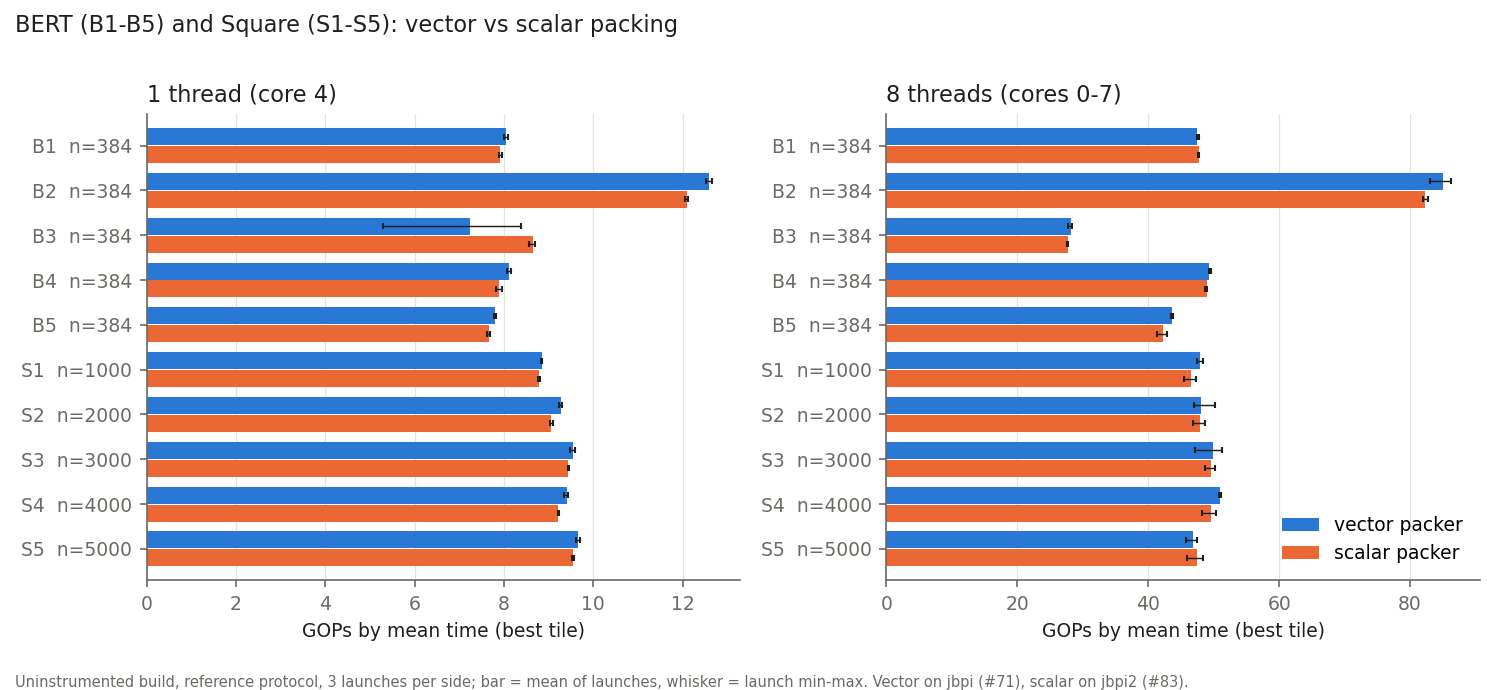
\includegraphics[width=\textwidth]{fig1_paper_vector_vs_scalar.png}\end{center}
\begin{center}
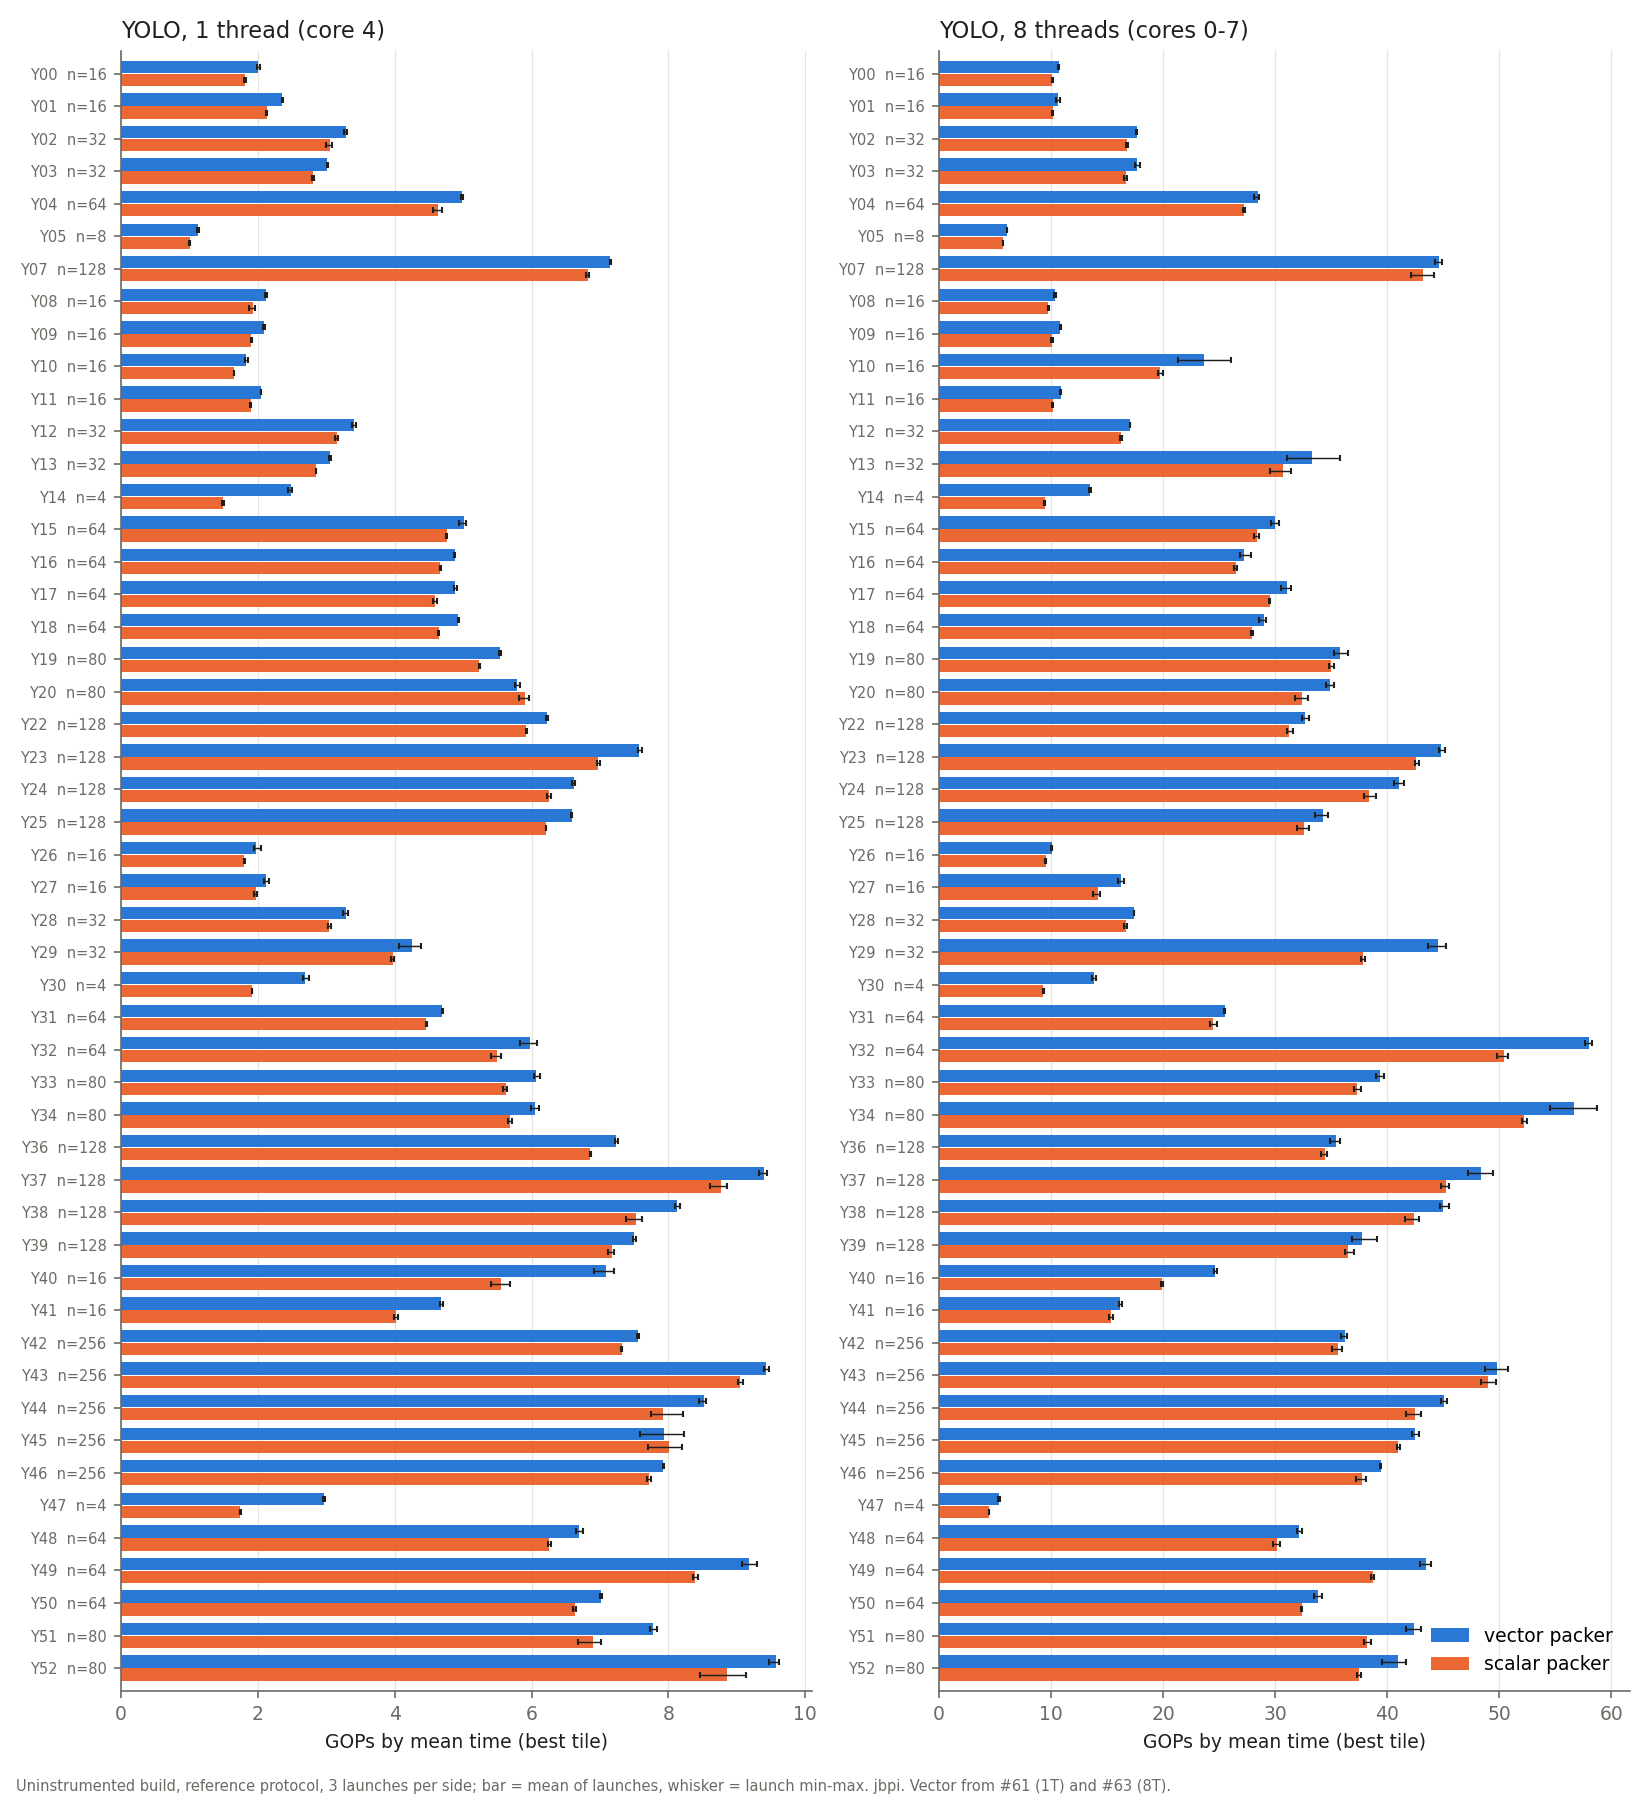
\includegraphics[width=\textwidth,height=0.85\textheight,keepaspectratio]{fig2_yolo_per_layer.png}
\end{center}

\section*{Part 2: why the shape and the reuse decide}
A GEMM packs a block of A ($m\times k$) once; each packed element then meets $n$ columns of B. Packing is about $mk$
copies against $2mnk$ flops, so its weight falls as $1/n$. BERT ($n=384$) and Square ($n\ge1000$) use each packed
element hundreds of times; YOLO layers mostly have $n=16$--$128$, three have $n=4$ (and $k=16$: calls of
microseconds).

\small
\begin{tabular}{@{}lcccccccccc@{}}
\toprule
scalar/vector (median) & $n=4$ & 8 & 16 & 32 & 64 & 80 & 128 & 256 & 384 & 1000--5000 \\
\midrule
YOLO 1T & 0.601 & 0.894 & 0.906 & 0.928 & 0.941 & 0.933 & 0.945 & 0.968 & & \\
YOLO 8T & 0.699 & 0.939 & 0.939 & 0.947 & 0.954 & 0.925 & 0.951 & 0.966 & & \\
BERT/Square 1T & & & & & & & & & 0.982 & 0.976--0.995 \\
BERT/Square 8T & & & & & & & & & 0.983 & 0.971--1.012 \\
\bottomrule
\end{tabular}
\normalsize

\begin{center}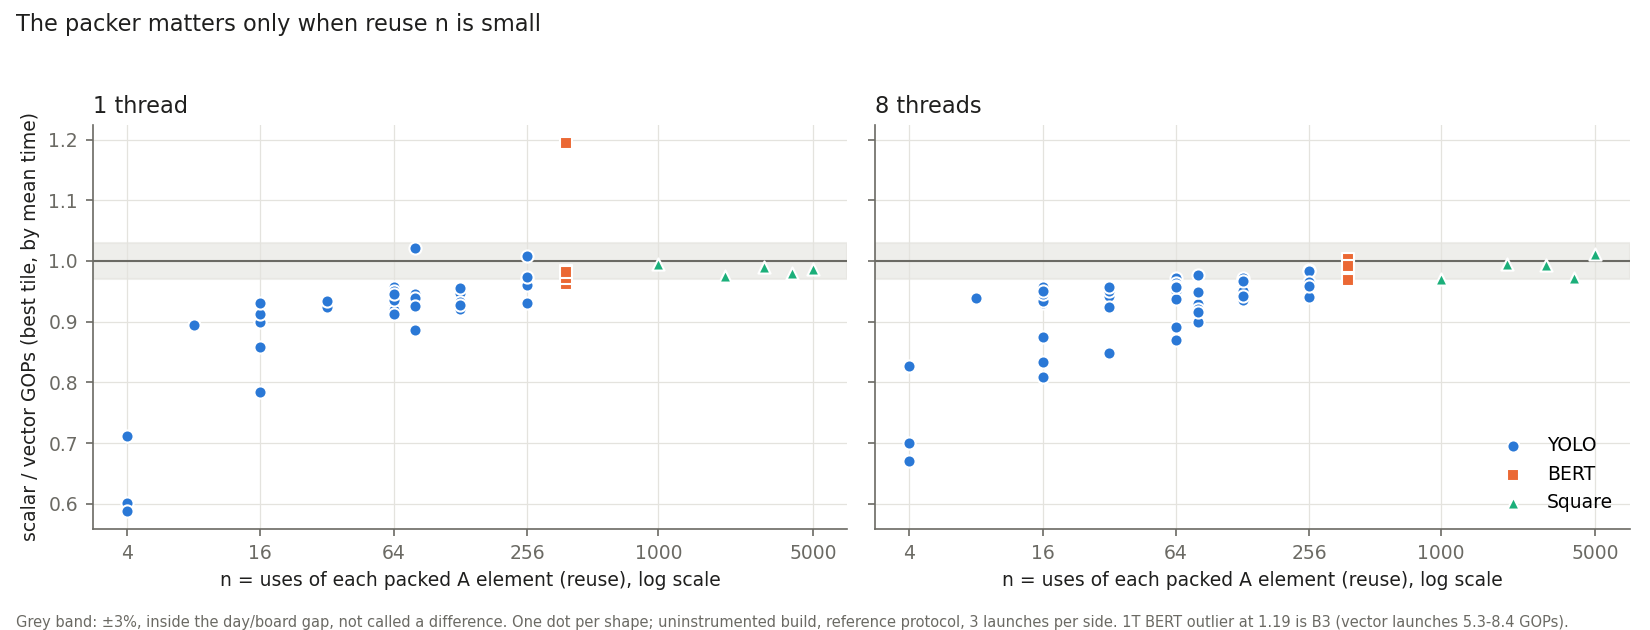
\includegraphics[width=\textwidth]{fig3_ratio_vs_reuse_n.png}\end{center}

\subsection*{T4: the measured pack share}
Instrumented build, warm-up protocol, 200 reps, 1T core 4, \texttt{jbpi2}, 4 launches (vector, scalar, scalar,
vector), each shape on its 1T best tile. Pack time covers A and B packing; means of 2 launches per packer.
``Predicted'' = (vector pack + compute) / (scalar pack + compute).

\small
\begin{tabular}{@{}llrrrrr@{}}
\toprule
shape & $m\times n\times k$ & pack share vec / scal & scal/vec pack time & predicted & measured (1T) \\
\midrule
Y14 & 4800x4x16 & 75\% / 83\% & 1.59 & 0.697 & 0.601 \\
Y30 & 1200x4x16 & 65\% / 74\% & 1.58 & 0.738 & 0.712 \\
Y47 & 300x4x16 & 51\% / 66\% & 1.94 & 0.667 & 0.589 \\
Y10 & 4800x16x32 & 77\% / 80\% & 1.15 & 0.899 & 0.900 \\
Y40 & 300x16x144 & 36\% / 50\% & 1.76 & 0.794 & 0.784 \\
Y29 & 1200x32x64 & 56\% / 60\% & 1.16 & 0.926 & 0.934 \\
Y19 & 4800x80x64 & 49\% / 52\% & 1.13 & 0.943 & 0.945 \\
Y42 & 300x256x1152 & 23\% / 25\% & 1.12 & 0.971 & 0.968 \\
B1 & 1024x384x1024 & 17\% / 19\% & 1.13 & 0.986 & 0.983 \\
B2 & 384x384x64 & 7\% / 10\% & 1.55 & 0.970 & 0.961 \\
S1 & $1000^3$ & 9\% / 9\% & 1.07 & 0.996 & 0.995 \\
\bottomrule
\end{tabular}
\normalsize

\begin{itemize}
  \item \textbf{Pack share follows $n$}: 49--83\% at $n=4$--80, 7--23\% at $n=256$--1000. It is far above $1/(2n)$
        because packing is memory-bound and the microkernel is not.
  \item \textbf{Scalar pack costs 1.07--1.16$\times$} on large, memory-bound packs, and \textbf{1.55--1.94$\times$} on small
        packs that stay in cache, where the vector packer's 8 floats per instruction win.
  \item \textbf{Total effect = pack share $\times$ extra pack cost.} BERT/Square: 7--19\% $\times$ 1.07--1.13 gives
        1--2\%, inside the noise. YOLO $n=4$: 51--75\% $\times$ 1.6--1.9 gives 26--40\%.
  \item The prediction matches within 1\% on 9 of 11 shapes. The misses are $n=4$ shapes (Y14, Y47), where calls of
        16--540\,$\mu$s make the 11--17\% timer cost distort the split most.
  \item It also explains why YOLO at $n=128$--256 still loses 3--5\% while BERT loses 1--2\%: Y42 spends 23\% of its
        time packing, B1 17\%, S1 9\%.
  \item \textbf{Threads:} at 8T the $n=4$ gap shrinks (Y14 0.60$\to$0.70, Y47 0.59$\to$0.83): each thread packs only
        its own rows of A. The 8-thread path has no timers (\iss{56}), so this is inferred, not measured.
\end{itemize}

\begin{center}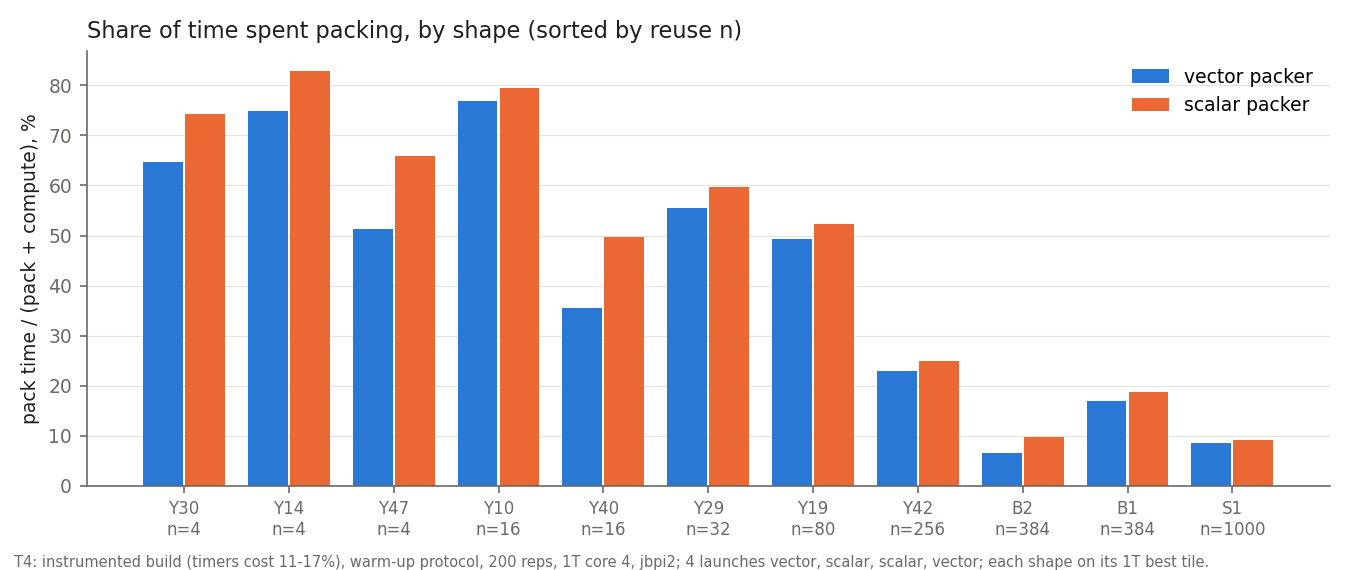
\includegraphics[width=0.85\textwidth]{fig4_pack_share_t4.png}\end{center}

\section*{Limits}
\begin{itemize}
  \item \textbf{Different days.} Vector runs 15--17 Nov, scalar runs 17 Nov, not interleaved: gaps under about 3\% are
        not called a difference. Day-drift check: H\'ector's unchanged \texttt{gemm.x} on \texttt{jbpi}, 17 Nov over
        16 Nov, median per layer 0.991 (sum of 50 layers 1223.5 $\to$ 1195.9 GFLOPS, 3 launches each).
  \item \textbf{Different boards for the paper part.} Vector on \texttt{jbpi} (\iss{71}), scalar on \texttt{jbpi2}:
        same SoC, but a board gap adds to the day gap.
  \item \textbf{T4 is instrumented}, on \texttt{jbpi2}: only its time shares and pack-time ratios are used.
  \item \textbf{Two packers, not packing against no packing.}
\end{itemize}

\end{document}
